\documentclass[a4paper]{article}

\usepackage[utf8]{inputenc}
\usepackage{graphicx}

\pdfimageresolution=108

\author{Adrien Nader}
\title{Introduction tutorial to Yellow Yeti Pkg, a fast, portable and inobstrusive package manager}

\begin{document}

\maketitle

\tableofcontents
\section{Installation}
\subsection{Dependencies}
Currently, yypkg depends on:
\begin{itemize}
  \setlength{\parskip}{0em}
  \item{ocaml-fileutils}: a library that provides the functionnality of the coreutils package under unices.
  \item{sexplib}: automated creation of type-safe serialization/deserialization functions from type definitions. All serialization functions in yypkg rely on it.
  \item{lablgtk2}: used for the gui, not a strong dependency.
\end{itemize}

\subsection{Windows}
\subparagraph{} It is advised to build under windows with the 'preprocessed\_src' folder and the 'BUILDING.windows' script (chmod +x it).

\subparagraph{} Support for windows is a bit "dirty". That doesn't mean it's bad, it only means that fileutils and sexplib (and type-conv) have to be put in \$(ocamlc -where) and lablgtk2 in \$(ocamlc -where)/lablgtk.\\
Also, findlib is not supported (the usual 'make' should work if you have everything setup, including camlp4, of course).

\subparagraph{} Note that there is a script ('preprocess.sh') to process the source files through camlp4 without compiling them, therefore producing files which can be compiled without camlp4 (mostly useful for windows).\\
You don't have to run it to use or compile yypkg but if you make changes to the src/ folder, they won't be propagated into preprocessed\_src automatically, and won't be seen when running BUILDING.windows.

\section{YYPREFIX and -prefix}
Since yypkg works in its own prefix, you need to tell it its value. This can be done in two ways: the YYPREFIX environment variable, or the -prefix switch to command-line arguments. It is advised to use YYPREFIX.

With most shells, run: export YYPREFIX=/path/to/your/prefix. The path can be absolute or relative.

On windows, in cmd.exe, run: set YYPREFIX=C:/path/to/your/prefix. Both forward and backward slashes work. You can also set it globally in System Properties.

From now on, we assume that you've set YYPREFIX.

\section{Initialisation}
\subsection{-init}
First, run yypkg -init. This will install some files, mostly create default settings and an empty package database.

On windows, it will also copy binaries to sbin/ so these can always be found (wget, bsdtar, liblzma...).

\begin{verbatim}
~/yypkg % export YYPREFIX=$(pwd)/prefix
~/yypkg % ./src/yypkg.native -init
~/yypkg % find prefix \! -type d | xargs ls -lh         
-rw-r--r-- 1 tux users 134 Dec 26 22:17 prefix/etc/yypkg.d/sherpa.conf
-rw-r--r-- 1 tux users  12 Dec 26 22:17 prefix/etc/yypkg.d/yypkg.conf
-rw-r--r-- 1 tux users   2 Dec 26 22:17 prefix/var/log/packages/yypkg_db
\end{verbatim}

\subsection{-config -setpreds}
Now, you have to tell yypkg which architectures it should accept for the packages. For instance, for win32 packages, you'll use 'i686-w64-mingw32'.
\begin{verbatim}
~/yypkg % ./src/yypkg.native -config -setpreds arch=noarch,i686-w64-mingw32
\end{verbatim}

And for win64 packages (there are no win64 packages currently so don't use yet):

\begin{verbatim}
~/yypkg % ./src/yypkg.native -config -setpreds arch=noarch,x86_64-w64-mingw32
\end{verbatim}

\section{sherpa-gui}
All the functions in yypkg are accessible from command-line and a graphical interface named sherpa (the sherpa carries packages to the yeti...).

\begin{center}
  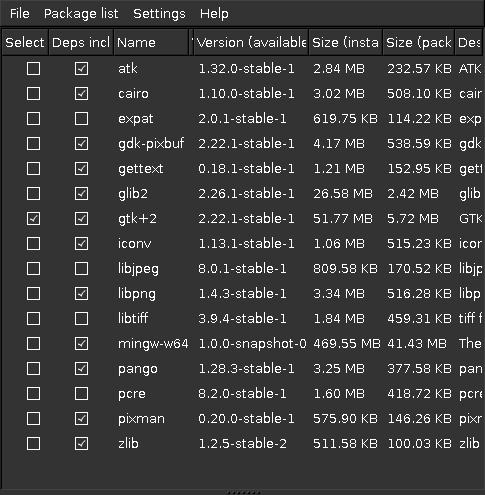
\includegraphics{../screenshots/sherpa_gui_1.png}
\end{center}

\subsection{Starting}
Currently, you should always start sherpa\_gui from a terminal since it'll write a lot to stdout/stderr. Also, you have to start it with the -sherpa parameter:
\begin{verbatim}
sherpa_gui -sherpa
\end{verbatim}

\subsection{Getting the package list}
Once it is started, go to Package List -> Force Update. You will be presented with a list of packages in a column layout. Most things are obvious so we'll only explain what goes with the 'Selected' and 'Deps included' columns.

\subsection{One word about package selection and dependencies}
YYPkg uses a very simple algorithm to manage dependencies.  Here, 'Selected' means that {\bf you} selected a package. When you do, the 'Deps included' column is update to reflect which packages the items that you selected depend on.\\
If you do not want a package that is ticked in the 'Deps included' column, simply untick it.\\

The dependencies are merely suggested, there is nothing to guarantee that all dependencies are met and nothing to 'force' one of them.

During uninstallation, the dependencies are simply not involved at all.

\subsection{Processing}
Once you are done, with the selection, go to File -> Process. Packages will be downloaded, installed for the ones that are selected and uninstalled for those that have to be.

There is currently no supported for updating a package: uninstall the old one and install the new one. This will be fixed shortly.

\section{Command-line tools: yypkg and sherpa}
These tools are not described in this document: see the 'USAGE' file for their usage.

\end{document}

